\begin{frame}{Resultados - Solución exacta de la ecuacion a(e)}
    Integrano la ecuación \ref{eq:dade}, encontramos que:
\begin{align*}
    \int_{a_{0}}^{a}\frac{d\bar{a}}{\bar{a}}&=\int_{e_{0}}^{e}\frac{12}{19}\frac{1+(73/24)\bar{e}^2+(37/96)\bar{e}^4}{\bar{e}(1-\bar{e}^2)[1+(121/304)\bar{e}^2]}\,d\bar{e},\\
    \ln \left(\frac{a}{a_{0}}\right)&=\int_{e_{0}}^{e}\frac{12}{19}\frac{1+(73/24)\bar{e}^2+(37/96)\bar{e}^4}{\bar{e}(1-\bar{e}^2)[1+(121/304)\bar{e}^2]}\,d\bar{e}.
\end{align*}
Despejando $a$, obtenemos la expresión
\begin{equation}
    \bar{a}= a_{0}\exp\left[\int_{e_{0}}^{e}\frac{12}{19}\frac{1+(73/24)\bar{e}^2+(37/96)\bar{e}^4}{\bar{e}(1-\bar{e}^2)[1+(121/304)\bar{e}^2]}\,d\bar{e}\right].
    \label{eq:bara}
\end{equation}
\end{frame}
\begin{frame}{Resultados - Solución exacta de la ecuacion a(e)}
    Calculando la integral en la expresión anterior con la libreria \textit{sympy} de \textit{python}, se obtiene
\begin{eqnarray*}
        \bar{a}=a_0exp\left[\frac{12}{19}log(e)-\frac{12}{19}log(e_0)-log(e^2-1)+\frac{870}{2299}log\left(e^2+\frac{304}{121}\right)\right.\\
        \left.+log\left(e^2_0-1\right)-\frac{870}{2299}log\left(e^2_0+\frac{304}{121}\right)\right]
\end{eqnarray*}
\begin{equation}
    \bar{a}= \frac{a_0e^{\frac{12}{19}}\left(e^2+\frac{304}{121}\right)^{\frac{870}{2299}}\left(e^2_0-1\right)}{e^{\frac{12}{19}}_0\left(e^2-1\right)\left(e_0^2+\frac{304}{121}\right)^{\frac{870}{2299}}}
\end{equation}
\end{frame}
\begin{frame}{Resultados - Solución exacta de la ecuacion a(e)}
    Si definimos a 
\begin{equation}
    g(e):= \frac{e^{\frac{12}{19}}}{1-e^2} \left(1+\frac{121}{304}\right)^{\frac{870}{2299}}
    \label{eq:g(e)}
\end{equation}
entonces, la solución puede escribirse como 
\begin{equation}
    a(e)= a_0\frac{g(e)}{g(e_0)}
    \label{eq:a(e)}
\end{equation}
\end{frame}
\begin{frame}{Resultados - Solución númerica de la ecuacion a(e)}
    Usando la siguiente adimencionalización \cite{Vito2008,Gonzalez2018,Gonz2019} de las variables
\begin{equation*}
    \tilde{a}:= \frac{a}{R_*}, \qquad  \tilde{t}:=\frac{ct}{R_*}.
\end{equation*}
donde
\begin{equation*}
    R_*^3 := \frac{4G^3\mu M^2}{c^6}.
\end{equation*}
Por lo tanto, las ecuaciones \ref{eq:dadt} y \ref{eq:dedt} son:
\begin{align}
    \label{eq:dadt2}
    \frac{d\tilde{a}}{d\tilde{t}} &= -\frac{16}{5}\frac{1}{\tilde{a}^3}\frac{1}{\left(1-e^2\right)^{7/2}}\left(1+\frac{73}{24}e^2+\frac{37}{96}e^4\right) ,\\
    \label{eq:dedt2}
\frac{de}{d\tilde{t}} &= -\frac{76}{15}\frac{1}{\tilde{a}^4}\frac{e}{\left(1-e^2\right)^{5/2}}\left(1+\frac{121}{304}e^2\right) .
\end{align}
\end{frame}
\begin{frame}{Resultados - Solución númerica de la ecuacion a(e)}
    \begin{figure}[H]
        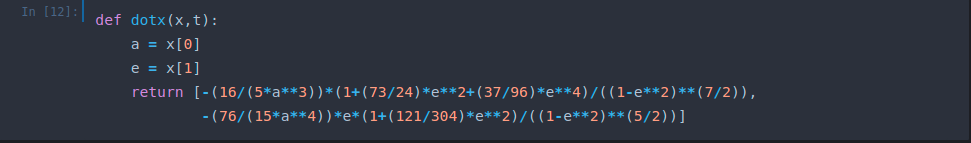
\includegraphics[scale=0.4]{images/dot.png}
        \caption{Función escrita en python que define la ecuación \ref{eq:dadt2} }
    \end{figure}
\end{frame}
\begin{frame}{Resultados - Solución númerica de la ecuacion a(e)}
    \begin{figure}[H]
        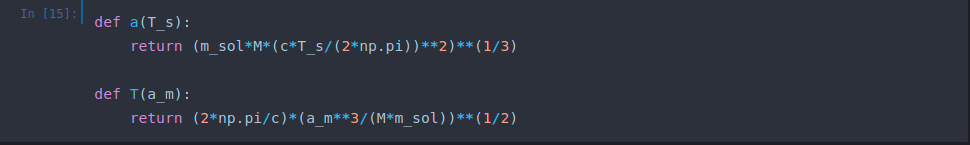
\includegraphics[scale=0.4]{images/fun.png}
        \caption{Función escrita en python que define la dependencia entre el periodo y el semieje mayor}
    \end{figure}
\end{frame}
\begin{frame}{Resultados - Solución númerica de la ecuacion a(e)}
    \begin{figure}[H]
        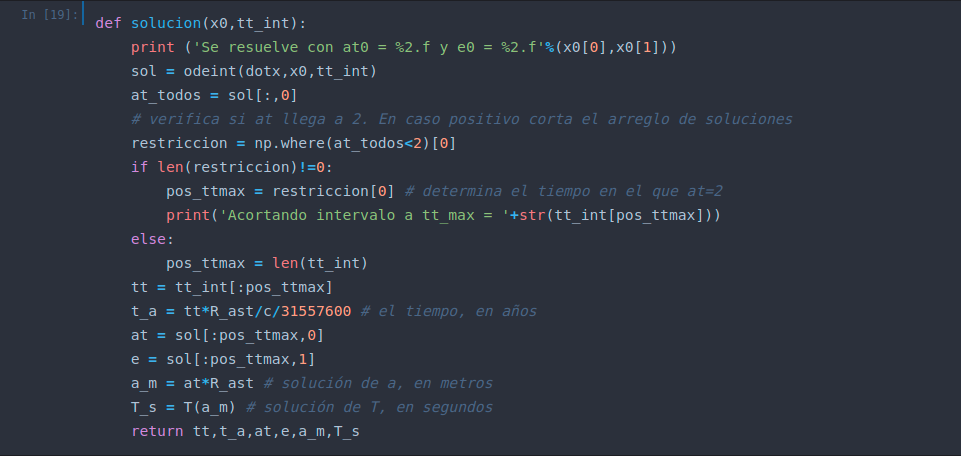
\includegraphics[scale=0.37]{images/solucion.png}
        \caption{Función que define la solución númerica del sistema binario}
    \end{figure}
\end{frame}
\begin{frame}{Resultados - Solución númerica de la ecuacion a(e)}
    \begin{minipage}{0.45\linewidth}
        \begin{figure}[H]
            \centering
            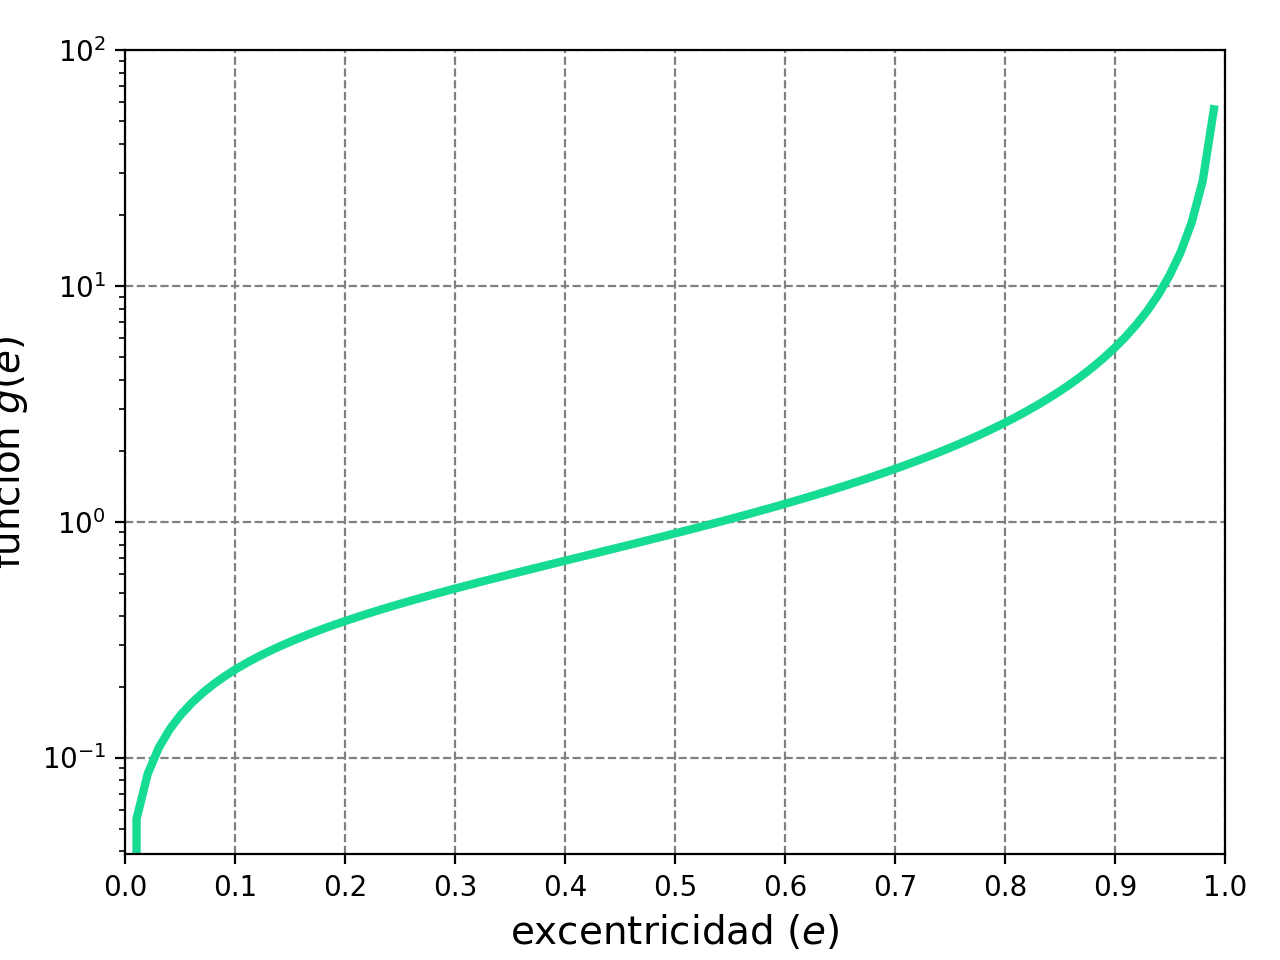
\includegraphics[height=4.5cm]{images/gvse.png}
            \caption{Función g(e) con respecto los valores de la excentricidad calculados.}
            \label{fig:gvse}
        \end{figure} 
    \end{minipage}
    \begin{minipage}{0.5\linewidth}
    \begin{figure}[H]
        \centering
        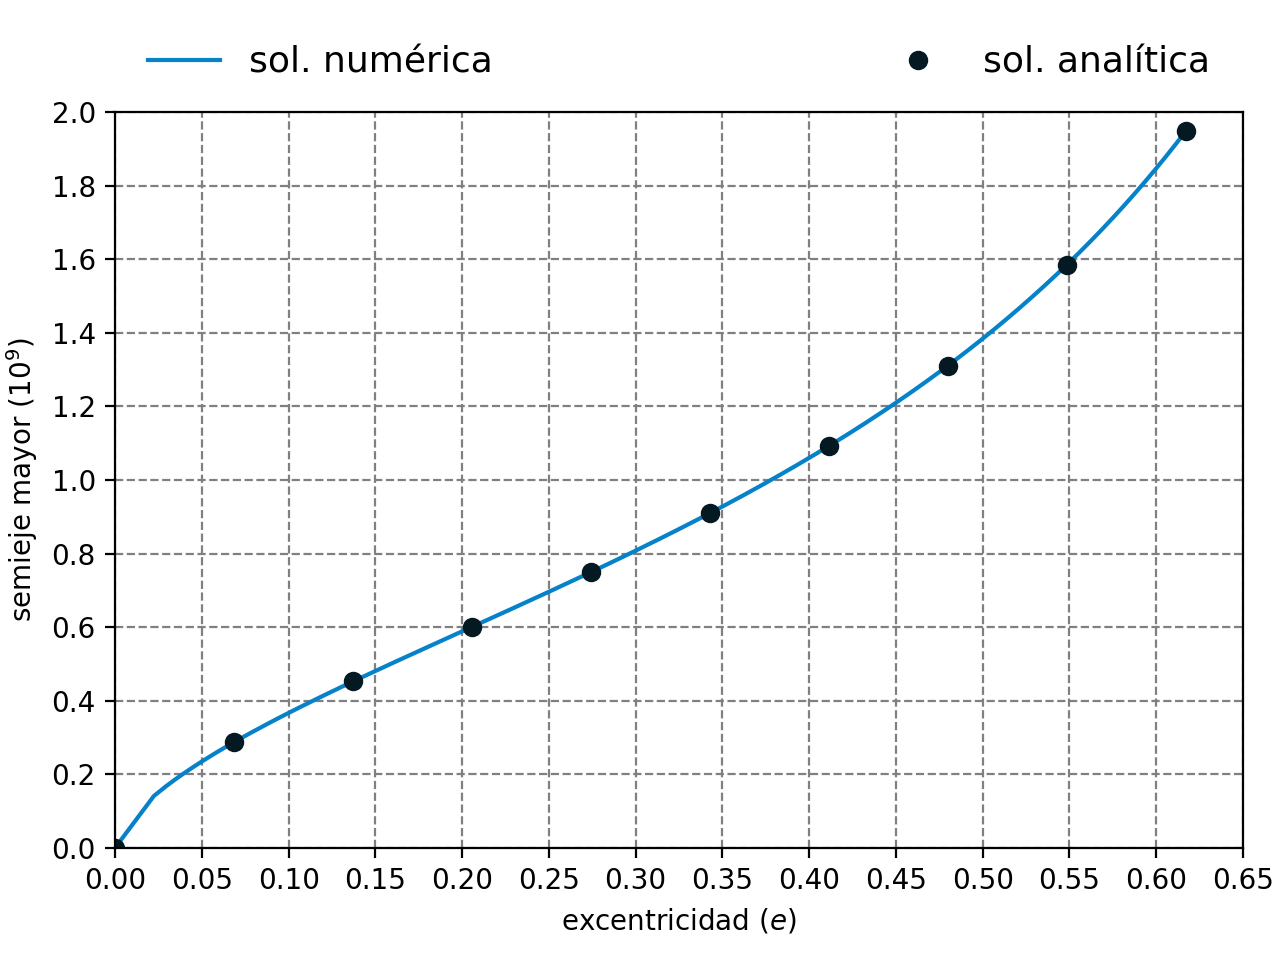
\includegraphics[height=4.5cm]{images/solana_solnum.png}
        \caption{Valores del semieje mayor $a$ con respecto a los valores de excentricidad $e$ para la solución analítica u numérica.}
        \label{fig:ananum}
    \end{figure}
    \end{minipage}
\end{frame}
\begin{frame}{Resultados - Solución númerica de la ecuacion a(e)}
    \begin{minipage}{0.5\linewidth}
        \begin{figure}[H]
            \centering
            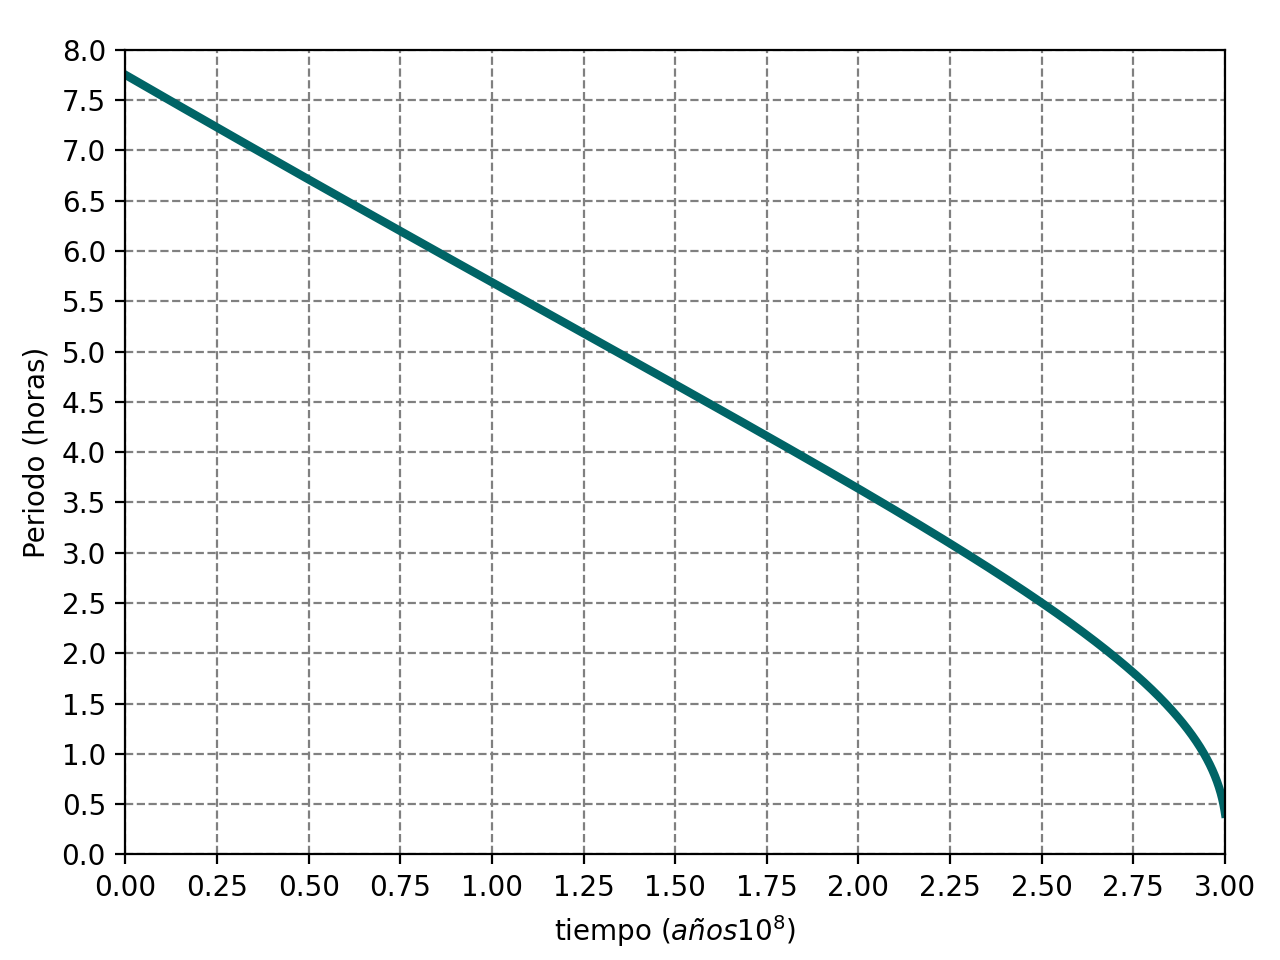
\includegraphics[height=5cm]{images/periodo.png}
            \caption{Periodo orbital en horas del sistema binario con respecto el tiempo en años.}
            \label{fig:periodo}
        \end{figure}
    \end{minipage}
    \begin{minipage}{0.45\linewidth}
        \begin{figure}[H]
            \centering
            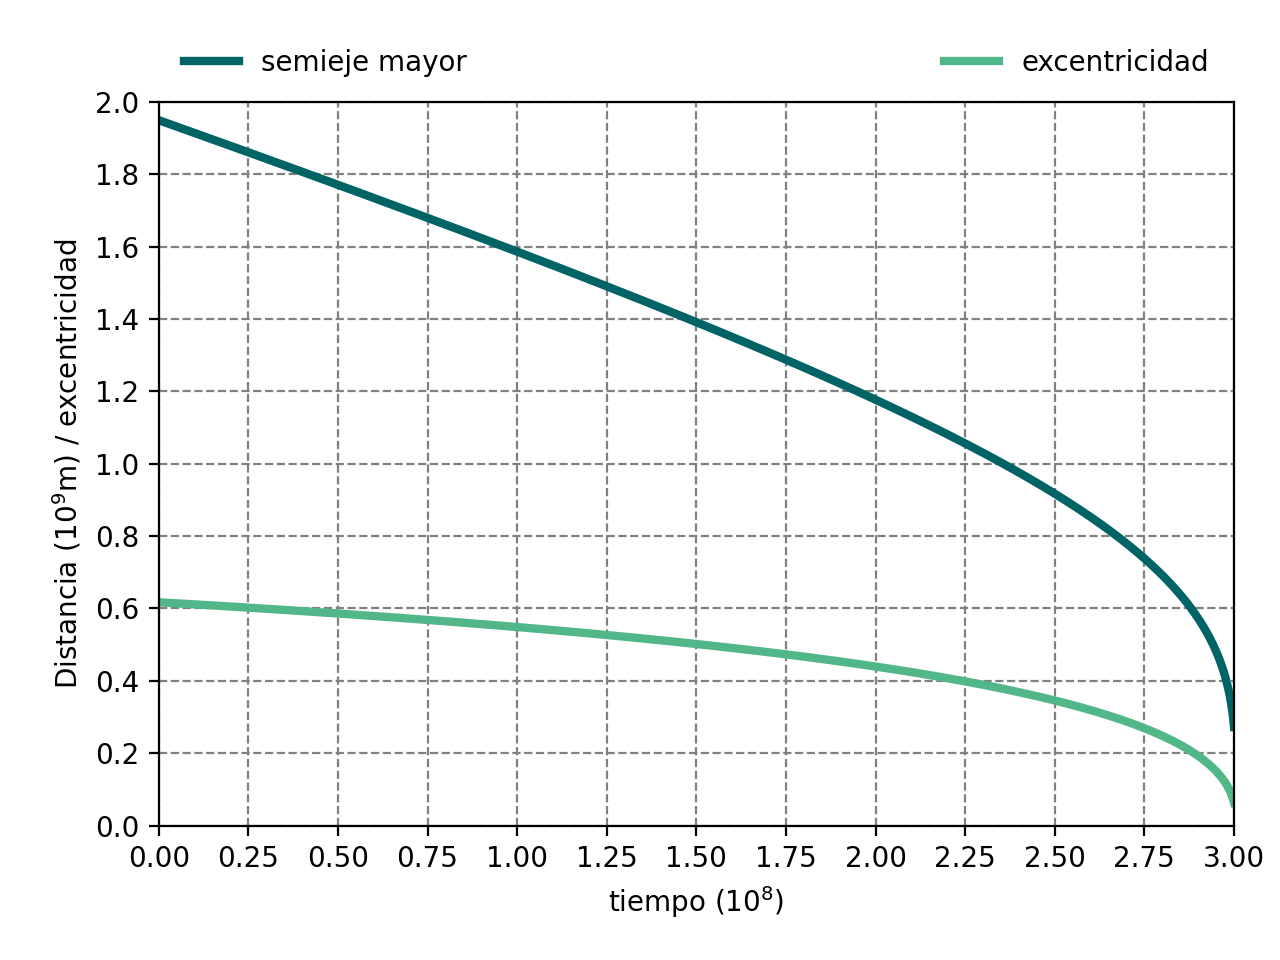
\includegraphics[height=5cm]{images/a_adim.png}
            \caption{Semieje mayor y la excentricidad de la dinámica del pulsar binario a lo largo del tiempo.}
            \label{fig:semieje,excentricidad}
        \end{figure} 
    \end{minipage}
\end{frame}
\begin{frame}{Resultados - Solución númerica de la ecuacion a(e)}
    \begin{align*}
        T(t)&\approx T_0 + \dot{T}(t-t_0),\\
        t_{n+1}& \approx t_n + T(t_n).
        \end{align*}
        que al ser iteradas implican que
        \begin{equation*}
        t_n \approx t_0+nT_0+\dot{T}T_0\frac{n(n-1)}{2}+O(\dot{T}{}^2).
        \end{equation*}
        Por lo tanto, el retardo respecto al valor newtoniano ($t_n^{\rm Newton}=t_0+nT_0$), luego de $n$ revoluciones es dado por
        \begin{equation*}
        (\Delta t)_n \approx \dot{T}T_0\frac{n(n-1)}{2}+O(\dot{T}{}^2).
        \end{equation*}
\end{frame}
\begin{frame}{Resultados - Solución númerica de la ecuacion a(e)}
    El valor de $\dot{T}$ puede ser evaluado usando la función \textcolor{def}{dotx} que definimos previamente, y con la relación
    \begin{equation*}
    \dot{T}=\frac{3}{2}\frac{c}{R_\ast}\frac{T}{\tilde{a}}\frac{d\tilde{a}}{d\tilde{t}}
    \end{equation*}
    Obteniendo un valor de 
    \begin{equation*}
        \frac{dT}{dt}=-2.402560x10^{-12}
    \end{equation*}
    Este valor concuerda con el reportado en \cite{Weisberg2010}. Por lo que comparando los datos observacionales con los teóricos obtenemos la figura \ref{fig:exp}.
\end{frame}
\begin{frame}{Resultados - Solución númerica de la ecuacion a(e)}
    \vspace{0.2cm}
    \begin{figure}[H]
        \centering
        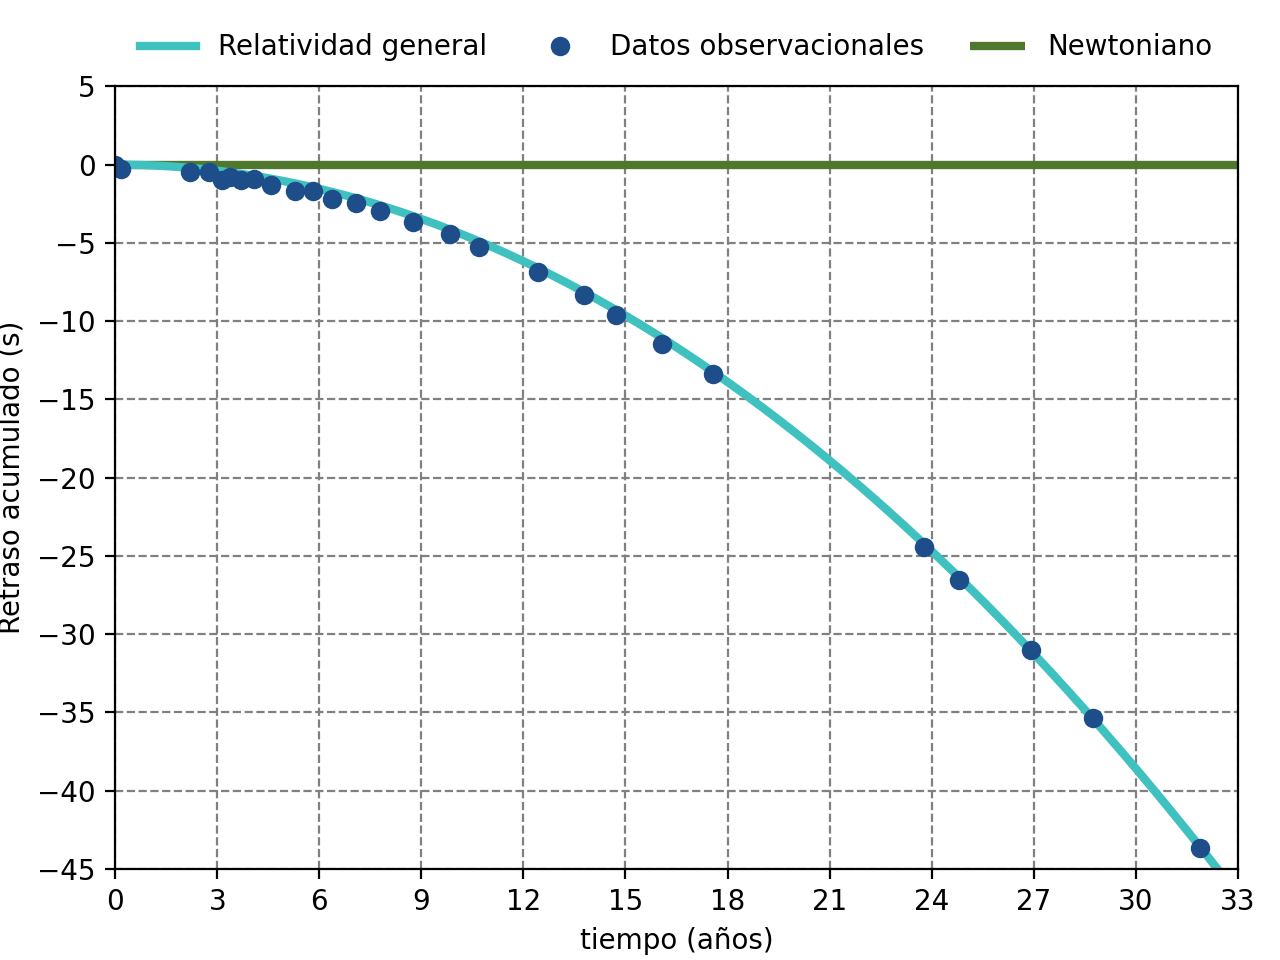
\includegraphics[scale=0.5]{images/exp.png}
        \caption{Datos observacionales reportados en \cite{Weisberg2010} comparados con la solución teórica aportada por la relatividad general y la teoría newtoniana.}
        \label{fig:exp}
    \end{figure}
\end{frame}